\ifdefined \wholebook \else\documentclass[oneside]{book}\usepackage{EdlBook}\graphicspath{{figures/}}
\addto\captionsicelandic{\renewcommand{\chaptername}{Kafli}}
%\setsecnumdepth{chapter}
\begin{document}
%%%
%
\setcounter{chapter}{14} % one less than this chapter
%
%%%
\fi
%%%%%%%%%%%%%%%%%%%%%%%%%%%%%%%%
%      CHAPTER TEXT GOES BELOW
%%%%%%%%%%%%%%%%%%%%%%%%%%%%%%%%

\renewcommand{\thefigure}{\arabic{figure}}
\counterwithout{equation}{chapter}

\chapter{Lögmál Gauss}

Áður en að við byrjum að fjalla um lögmál Gauss þá ættum við að skoða Maxwells-jöfnurnar fjórar:

\begin{align*}
    \begin{dcases*}
     \oint \Vec{E} \cdot d\Vec{A} = \frac{Q_{\text{inni}}}{\epsilon_0}, & \hspace{1cm} \emph{(Lögmál Gauss fyrir rafsvið)} \\
     \oint \Vec{B} \cdot d\Vec{A} = 0, & \hspace{1cm} \emph{(Lögmál Gauss fyrir segulsvið)} \\ 
     \oint \vec{E} \cdot d\vec{\ell} = - \frac{d\Phi_B}{dt}, & \hspace{1cm} \emph{(Lögmál Faradays)} \\
     \oint \vec{B} \cdot d \vec{\ell} = \mu_0 I_{\text{inni}}, & \hspace{1cm} \emph{(Lögmál Ampéres)}.
    \end{dcases*}
\end{align*}

Það kann kannski að koma ykkur spánskt fyrir sjónir að engin af jöfnunum hér á undan er kennd við Maxwell - en það er vegna þess að hann var fyrstur manna til þess að átta sig á því hvernig að þessar fjórar jöfnur tengjast (og að þær lýsi einu og sama fyrirbærinu). Reyndar var hans helsta framlag í öllu þessu máli að \educk{lagfæra} fjórðu jöfnuna (Lögmál Ampéres) þannig að hún yrði:
\begin{align*}
    \oint \vec{B} \cdot d\vec{\ell} = \mu_0 I_{\text{inni}} + \mu_0 \varepsilon_0 \frac{d\Phi_E}{dt}, \hspace{1cm} \text{\emph{(Lögmál Maxwells)}}.
\end{align*}
Það er reyndar fræg saga af Maxwell og Eureka-mómentinu hans þegar honum tókst að sýna fram á að ljós er rafsegulbylgja. Það tengist allt saman þeirri merkilegu staðreynd að ljóshraðinn er:
\begin{align*}
    c = \frac{1}{\sqrt{\mu_0 \varepsilon_0}} = \SI{3.00e8}{m/s}.
\end{align*}
Það er því einnig hægt að skrifa lögmál Maxwells á eftirfarandi formi:
\begin{align*}
    \oint \vec{B} \cdot d\vec{\ell} = \mu_0 I_{\text{inni}} + \frac{1}{c^2} \frac{d\Phi_E}{dt}, \hspace{1cm} \text{\emph{(Lögmál Maxwells)}}.
\end{align*}
Maxwells-jöfnurnar útskýra alla rafsegulfræði. Þær eru án efa hagnýttustu jöfnur mannkynssögunnar - þær eru fjórar og líta út fyrir að vera einfaldar (kannski finnst ykkur það ekki sem stendur en bíðiði bara!). Samt sem áður er fólk enn þann daginn í dag að afhjúpa leyndardóma Maxwellsjafnanna (t.d.~nýlega uppgötvuðu menn hvernig er hægt að hlaða síma án þess að stinga þeim í samband með því að leggja þá ofan á flöt sem að býr til segulsvið sem að er hægt að nota til þess að hlaða rafhlöðuna). Við skulum því hefjast handa við það að skoða Maxwells-jöfnurnar og byrjum því á þeirri fyrstu: Lögmál Gauss fyrir rafsvið.

\newpage

\section{Rafflæði}

Þegar við vorum að skoða flæði í vatnspípum þá töluðum við um flæðið í gegnum vatnspípuna sem stærðina $\Phi = Av$ þar sem $A$ var flatarmálið á pípunni og $v$ var straumhraði vatnsins þvert á flatarmálið. Við höfðum þá sýnt að vatnsflæði í pípum er varðveitt, þ.e.a.s.~$A_1v_1 = A_2 v_2$ eða með öðrum orðum $\Phi = \text{fasti}$. Nú kynnum við hinsvegar til sögunnar almennara stærðfræðilegt hugtak fyrir flæði. Við viljum nefnilega geta talað um rafflæði:

\begin{tcolorbox}
\begin{definition}
Lítum á hlut með flatarmál $\vec{A}$ þar sem að \\ rafsviðið er gefið með $\vec{E}$. Látum $\theta$ vera hornið á milli vigranna. \\ \textbf{Rafflæðið} út um flötinn er þá gefið með:
\begin{align*}
    \Phi_E = \vec{E} \cdot \vec{A} = EA\cos\theta
\end{align*}
\end{definition}
\vspace{-2.75cm}
\begin{figure}[H]
    \hspace{11cm}
    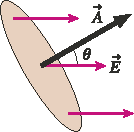
\includegraphics{rafflaedinn.pdf}
\end{figure}
\end{tcolorbox}

\vspace{0.2cm}

\begin{minipage}{\linewidth}

\begin{wrapfigure}{r}{2.3in}
\vspace{0.4cm}
\centering
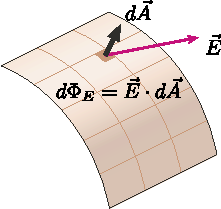
\includegraphics{figures/orsmaedarflaedi.pdf}
\end{wrapfigure}


Stundum viljum við setja þetta fram á örsmæðarformi. Til dæmis ef að yfirborðið okkar er kúpt eða bogið. Þá skiptum við flatarmálinu upp í örsmæðir $d\vec{A}$ og skoðum örrafflæðið út um sérhvert örsmæðarflatarmál. Við skrifum þá $d\Phi_E = \vec{E} \cdot d\vec{A}$. Við þurfum síðan að leggja saman framlagið frá öllum þessum örrafflæðum til þess að finna heildarrafflæðið. En þá er:
\begin{align*}
    \Phi_E = \oint d \Phi_E = \oint \vec{E} \cdot d\vec{A}.
\end{align*}
Þar sem að $\oint$ táknar tegur yfir allt yfirborð hlutarins. Yfirborð hlutarins sem að við erum að tegra yfir kallast \emph{Gauss-flötur}. Við veljum oft ímyndaða Gauss-fleti (lögmál Gauss gildir líka um þá!). Lögmál Gauss segir þá einfaldlega að rafflæðið er varðveitt:
\end{minipage}

\vspace{0.2cm}


\begin{tcolorbox}
\begin{theorem}
\textbf{(Lögmál Gauss)} Lítum á hlut með rúmmál $V$ og yfirborðsflatarmál $A$. Látum hlutinn umlykja heildarhleðslu $Q_{\text{inni}} = Q_1 + Q_2 + \ldots + Q_n$. Þá gildir að:
\begin{align*}
    \Phi_E = \oint \vec{E} \cdot d\vec{A} = \frac{Q_{\text{inni}}}{\varepsilon_0}.
\end{align*}
\end{theorem}
\end{tcolorbox}


Við skulum núna sanna/leiða út lögmál Coulombs með því að nota lögmál Gauss:

\begin{tcolorbox}
\begin{theorem}
\textbf{(Lögmál Gauss} $\mathbf{\implies}$ \textbf{Lögmál Coulombs)} Lítum á punkthleðslu $Q$. Þá er rafsviðið í fjarlægð $r$ frá punkthleðslunni gefið með $E(r) = \frac{kQ}{r^2}$. Sér í lagi gildir að rafkrafturinn sem að jákvæð prufuhleðsla, $+q$, finnur fyrir í fjarlægð $r$ frá punkthleðslunni er gefinn með $F_k = qE = \frac{kQq}{r^2}$.
\end{theorem}
\end{tcolorbox}

\textbf{Útleiðsla:} Til þess að nota lögmál Gauss þurfum við fyrst að velja Gauss-flöt. Við veljum Gauss-flötinn okkar sem kúluna með geisla $r$ í kringum punkthleðsluna, $Q$. Þá fæst samkvæmt lögmáli Gauss að:
\begin{align*}
    \Phi_E = \oint \vec{E} \cdot d\vec{A} = \frac{Q_{\text{inni}}}{\varepsilon_0} \implies E \explain{\oint dA}{4\pi r^2} = \frac{Q}{\varepsilon_0} \implies E \cdot 4\pi r^2 = \frac{Q}{\varepsilon_0} \implies E(r) = \frac{1}{4\pi \varepsilon_0} \frac{Q}{r^2} = \frac{kQ}{r^2}.
\end{align*}
Hér höfum við notað að rafsviðið og þverilvigur yfirborðsins eru alltaf samsíða (svo hornið á milli þeirra er núll). Vegna samhverfu er gildið á rafsviðinu $\vec{E}$ alltaf það sama í fjarlægð $r$ frá punkthleðslunni svo að það er fasti fyrir sérhvern smábút $dA$ og við getum því tekið það út fyrir tegrið. Loks notuðum við að $k = \frac{1}{4\pi \varepsilon_0}$. \qed

\begin{tcolorbox}
\begin{theorem}
\textbf{(Rafsvið frá plötu)} Skoðum plötu með flatarmál $A$ og jafndreifða hleðslu $Q$. Þá er rafsviðið frá plötunni gefið með:
\begin{align*}
    E_{\text{plata}} = \frac{Q}{2\varepsilon_0 A}.
\end{align*}
\end{theorem}
\end{tcolorbox}

\begin{minipage}{\linewidth}

\begin{wrapfigure}{r}{2.3in}
\vspace{0.4cm}
\centering
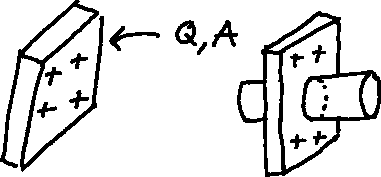
\includegraphics{figures/sivaln-hdrawn.pdf}
\end{wrapfigure}

\textbf{Útleiðsla:} Hleðsluþéttleiki plötunnar er $\sigma = \frac{Q}{A}$. Velum nú Gauss-flöt sem er sívalningur sem nær í gegnum báðar hliðar og hefur lengd $\ell$ og geisla $r$ þar sem $r \ll \sqrt{A}$ og lengdin er meiri heldur en þykkt plötunnar. Hver er þá hleðslan inni í Gauss-fletinum? Hún er:
\begin{align*}
    Q_{\text{inni}} = \sigma r^2 \pi 
\end{align*}
En þar með höfum við samkvæmt lögmáli Gauss að:
\begin{align*}
    \Phi_E = \oint \vec{E} \cdot d\vec{A} = \frac{Q_{\text{inni}}}{\varepsilon_0} = \frac{\sigma r^2 \pi}{\varepsilon_0}.
\end{align*}
En hvert er rafflæðið út um Gauss-flötinn? Við sjáum að rafsviðið verður að liggja beint frá plötunni í báðar stefnur (ef $Q$ er jákvæð - annars liggja rafsviðslínurnar beint að plötunni) svo að það er ekkert rafflæði út um hliðar sívalningsins, það er einungis rafflæði út um botninn og topinn á sívalningnum. Við höfum þá að:
\begin{align*}
    \Phi_E = \explain{\Phi_{\text{hliðar}}}{= 0} + \Phi_{\text{toppur}} + \Phi_{\text{botn}} = E \pi r^2 + E\pi r^2 = 2\pi Er^2.
\end{align*}
Þar sem að við höfum notað að $\vec{E}$ og $\vec{A}$ eru samsíða fyrir bæði botninn og toppinn. En þar með ályktum við:
\begin{align*}
    \Phi_E = \oint \vec{E} \cdot d\vec{A} = \frac{Q_{\text{inni}}}{\varepsilon_0} \implies 2\pi r^2 E = \frac{\sigma r^2 \pi}{\varepsilon_0} \implies E_{\text{plata}} = \frac{\sigma r^2 \pi}{2\pi r^2 \varepsilon_0} = \frac{\sigma}{2 \varepsilon_0} = \frac{Q}{2\varepsilon_0 A}.
\end{align*}
\qed
\end{minipage}

Þetta er í rauninni frekar skrítin niðurstaða því að við fáum að rafsviðið er óháð fjarlægðinni frá plötunni. Þannig að í óendanlegri fjarlægð frá plötuþéttinum þá ætti rafsviðið einnig að vera gefið með $E_{\text{plata}} = \frac{Q}{2\varepsilon_0 A}$. Kannski hefði ég átt að minnast á það á einhverjum tímapunkti en við gerðum eiginlega ráð fyrir því að platan væri óendanlega stór í útleiðslunni! Það er þá spurning hvort að þetta sé góð nálgun eftir allt saman? Í rafsegulfræði þá er ágæt þumalputtaregla að ef að hluturinn er meira en \SI{5}{cm} á lengd þá er hann svo gott sem óendanlega langur (þ.e.~$\SI{5}{cm} \approx \infty$). En niðurstaðan hér á undan gefur okkur sniðuga leið til þess að leiða út eftirfarandi (sem við munum nota mikið í vetur!):

\newpage

\begin{tcolorbox}
\begin{theorem}
\textbf{(Rafsvið frá plötuþétti)} Lítum á tvær plötur með flatarmál $A$ sem eru í fjarlægð $d$ frá hvor annarri. Látum plöturnar hafa jafnstóra en gagnstæða hleðslu $\pm Q$. Þá er rafsviðið á milli platnanna gefið með:
\begin{align*}
    E_{\text{plötuþéttir}} = \frac{Q}{\varepsilon_0 A}.
\end{align*}
\end{theorem}
\end{tcolorbox}

\textbf{Útleiðsla:} Við byrjum á því að teikna upp mynd af plötuþéttinum:

\begin{figure}[ht!]
    \centering
    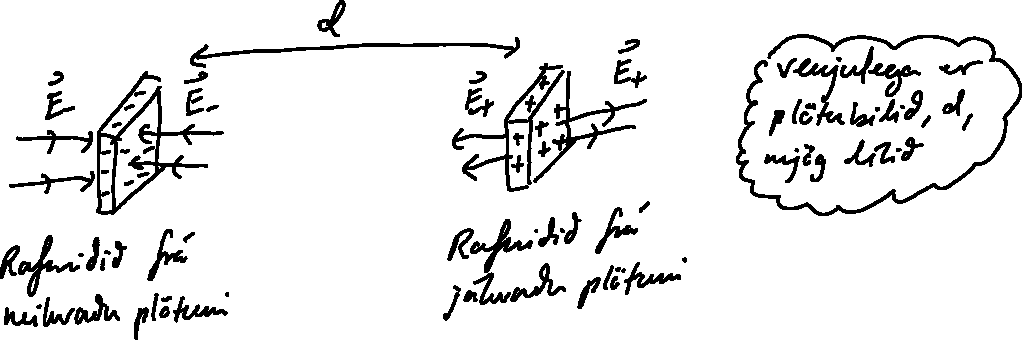
\includegraphics{figures/rafsvidid-plata.pdf}
\end{figure}

En við höfum þá eiginlega þrjú tilvik:

\begin{figure}[ht!]
    \centering
    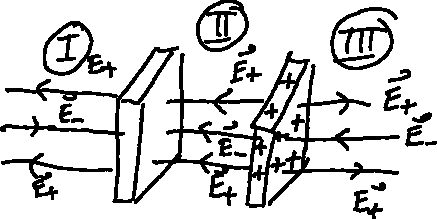
\includegraphics{figures/tilvik.pdf}
\end{figure}

Við sjáum þá að:
\begin{align*}
    E_\text{I} = E_- - E_+ = \frac{Q}{2\varepsilon_0 A} - \frac{Q}{2\varepsilon_0 A} = 0.
\end{align*}
og eins er
\begin{align*}
    E_{\text{III}} = E_+ - E_- = \frac{Q}{2\varepsilon_0 A} - \frac{Q}{2\varepsilon_0 A} = 0.
\end{align*}
En á milli platnanna höfum við að:
\begin{align*}
    E_{\text{II}} = E_+ + E_- = \frac{Q}{2\varepsilon_0 A} + \frac{Q}{2\varepsilon_0 A} = \frac{Q}{\varepsilon_0 A}.
\end{align*}
Þannig að við álytum að $E_{\text{plötuþéttir}} =  \frac{Q}{\varepsilon_0 A}$ á milli platnanna. \qed

\newpage

\begin{tcolorbox}
\begin{theorem}
\textbf{(Rafsvið frá löngum beinum vír)} Lítum á rafmagnsvír með geisla $R$ og lengd $L$ sem ber rafstraum þannig að heildarhleðslan inni í þessum vírbút er $Q$. Þá er rafsviðið frá vírnum gefið með:
\begin{align*}\hspace{-5cm}
    E_{\text{vír}} = \begin{cases} 
    \displaystyle \frac{Q}{2\pi \varepsilon_0 R^2 L}\cdot r & \text{ef $r \leq R$.} \\[3ex]
    \displaystyle\frac{Q}{2\pi \varepsilon_0 L} \cdot \frac{1}{r} & \text{ef $r > R$}.
    \end{cases}
\end{align*}
\end{theorem}
\vspace{-2.75cm}
\begin{figure}[H]
    \hspace{9cm}
    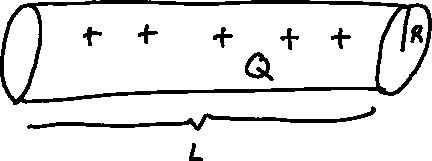
\includegraphics[scale = 0.7]{figures/sivaln-langrvir.pdf}
\end{figure}
\end{tcolorbox}

\textbf{Útleiðsla:} Byrjum á því að athuga að hleðsluþéttleiki vírsins er:
\begin{align*}
    \rho = \frac{Q}{\pi R^2 L}
\end{align*}
Skoða hvernig rafsviðið breytist inni í vírnum og fyrir utan. Veljum Gauss-flöt sem er sammiðja sívalningur með lengd $\ell < L$ og geisla $r$. Byrjum á því að skoða tilvikið þegar að $r > R$ (fyrir utan sívalninginn). Þá höfum við einfaldlega að:
\begin{align*}
    \Phi_{E} = \oint \vec{E} \cdot d\vec{A} = \explain{\Phi_{\text{hliðar}}}{E \cdot 2\pi r \ell} + \explain{\Phi_{\text{botn}}}{= 0} + \explain{\Phi_{\text{toppur}}}{= 0} = \frac{Q_{\text{inni}}}{\varepsilon_0} = \frac{\rho \pi R^2 \ell}{\varepsilon_0} \implies E(r) = \frac{\rho}{2\varepsilon_0} \cdot \frac{R^2}{r} = \frac{Q}{2\pi \varepsilon_0 L} \cdot \frac{1}{r}.
\end{align*}
Hinsvegar ef $r < R$ þá fæst að $Q_{\text{inni}} = \rho \pi r^2 \ell$ svo lögmál Gauss gefur að:
\begin{align*}
    \Phi_{E} = \oint \vec{E} \cdot d\vec{A} \implies E(r) \cdot 2\pi r \ell = \frac{\rho \pi r^2 \ell}{\varepsilon_0} = \frac{Q r^2 \ell}{\varepsilon_0 R^2 L} \implies E(r) = \frac{Q}{2\pi \varepsilon_0 L R^2} \cdot r.
\end{align*}

Að lokum getum við teiknað graf sem að sýnir þessa hegðun:


\begin{figure}[H]
    \centering
    \begin{tikzpicture}
      \draw[thick,-Stealth] (-2,0) -- (12,0);
      \draw[thick,-Stealth] (0,-1) -- (0,7);
      \draw[scale=1, domain=-0:5, smooth, variable=\x, blue] plot ({\x}, {\x});
      \draw[scale=1, domain=5:12, smooth, variable=\x, blue] plot ({\x}, {25/(\x)});
      \draw[thick] (5,-0.2) -- (5,0.2);
      \draw[thick] (-0.2,5) -- (0.2,5);
      \draw[dashed] (0.2,5) -- (5,5);
      \node at (0,7.5) {$E(r)\, \, [\si{N/C}]$};
      \node at (-0.95, 5) {$\frac{Q}{2\pi \varepsilon_0 R L}$};
      \node at (5,-0.5) {$r = R$};
      \node at (2.5,-0.5) {\emph{Inni í vírnum}};
      \node at (8.5,-0.5) {\emph{Fyrir utan vírinn}};
      \node at (12,-0.5) {$r \, \, [\si{m}]$};
      \draw[thick, -Stealth] (8,4) -- (7.3,3.6);
      \node at (9, 4.35) {$\frac{Q}{2\pi \varepsilon_0 L} \cdot \frac{1}{r} \xrightarrow[r \to \infty]{} 0$};
      \draw[thick, -Stealth] (2.25,3.75) -- (3,3.5);
      \node at (1.4,3.95) {$\frac{Q}{2\pi \varepsilon_0 L R^2} \cdot r$};
    \end{tikzpicture}
    \caption{Graf af styrk rafsviðsins frá löngum beinum vír með geisla $R$ í fjarlægð $r$ frá miðju vírsins.}
\end{figure}
Takið eftir að rafsviðsstyrkurinn frá vírnum ($\frac{1}{r}$) fellur hægar en rafsviðsstyrkurinn frá punkthleðslu ($ \frac{1}{r^2}$).

\section{Lögmál Gauss fyrir þyngdarsviðið (*)}

Þar sem að það er ákveðið samræmi á milli Coulombskraftsins og þyngdarlögmálskraftsins þá ættum við að geta fundið Gausslögmál fyrir þyngdarlögmálið. Höfum séð að:
\begin{align*}
    E(r) = \frac{1}{4\pi \varepsilon_0} \frac{Q}{r^2} \implies \Phi_E = \oint  \vec{E} \cdot d\vec{A} = \frac{Q_{inni}}{\varepsilon_0}.
\end{align*}
Ef þyngdarsviðið er táknað með $\vec{g}$ þá ættum við að hafa:
\begin{align*}
    g(r) = \frac{GM}{r^2} \implies \Phi_g = \oint \vec{g} \cdot d\vec{A} = 4\pi G M_{\text{inni}}.
\end{align*}
Við getum þá notað þetta til þess að skoða hvernig styrkur þyngdarsviðsins breytist inni í jörðinni eftir því sem að við förum neðar. Lítum því á jörðina sem einsleita kúlu með geisla $R$ og jafndriefðan massa $M$. Við viljum ákvarða þyngdarhröðunina inni í jörðinni fyrir $r < R$ og fyrir $r > R$. Fyrir $r > R$ fáum við einfaldlega að:
\begin{align*}
    \oint \vec{g} \cdot d\vec{A} = 4\pi GM \implies g(r) \cdot 4 \pi r^2 = 4\pi G M \implies g(r) = \frac{GM}{r^2}, \hspace{1cm} \text{fyrir $r > R$.}
\end{align*}
Hinsvegar ef $r < R$ þá þurfum við að ákvarða hvað $M_{\text{inni}}$ er (því núna er það ekki massi allrar jarðarinnar). Því er gott að nota eðlismassa jarðarinnar:
\begin{align*}
    \rho = \frac{M}{V} = \frac{M}{\frac{4\pi}{3} R^3}, \hspace{0.75cm} \text{þannig að} \hspace{0.5cm} M_{\text{inni}} = \rho V_{\text{inni}} = \rho \frac{4\pi}{3}r^3
\end{align*}
sem gefur því að $M_{\text{inni}} = M\left( \frac{r}{R} \right)^3$. Við fáum því að:
\begin{align*}
    \oint \vec{g}(r) \cdot d \vec{A} = 4\pi G M_{\text{inni}} \implies g(r) \cdot 4\pi r^2 = 4\pi G M \left( \frac{r}{R} \right)^3
\end{align*}
sem gefur því að:
\begin{align*}
    g(r) = \frac{GM}{R^2} \frac{r}{R}, \hspace{1cm} r < R.
\end{align*}
Sjáum sér í lagi að þegar $r = R$ þá er $g(r) = \frac{GM}{R^2}$ eins og við var að búast. Á næstu blaðsíðu má síðan sjá graf sem sýnir þyngdarhröðun jarðar sem fall af fjarlægð frá miðju jarðarinnar, $r$.

\newpage

\begin{figure}[H]
    \centering
    \begin{tikzpicture}
      \draw[thick,-Stealth] (-2,0) -- (12,0);
      \draw[thick,-Stealth] (0,-1) -- (0,7);
      \draw[scale=1, domain=-0:5, smooth, variable=\x, blue] plot ({\x}, {\x});
      \draw[scale=1, domain=5:12, smooth, variable=\x, blue] plot ({\x}, {125/(\x*\x)});
      \draw[thick] (5,-0.2) -- (5,0.2);
      \draw[thick] (-0.2,5) -- (0.2,5);
      \draw[dashed] (0.2,5) -- (5,5);
      \node at (0,7.5) {$g(r)\, \, [\si{m/s^2}]$};
      \node at (-0.75, 5) {$\frac{GM}{R^2}$};
      \node at (5,-0.5) {$r = R$};
      \node at (12,-0.5) {$r \, \, [\si{m}]$};
      \draw[thick, -Stealth] (8,4) -- (7,3);
      \node at (9, 4.25) {$\frac{GM}{r^2} \xrightarrow[r \to \infty]{} 0$};
      \draw[thick, -Stealth] (2.25,3.75) -- (3,3.5);
      \node at (1.5,3.95) {$\frac{GM}{R^3} \cdot r$};
    \end{tikzpicture}
    \caption{Graf af þyngdarhröðun jarðar sem fall af $r$.}
\end{figure}

Takið eftir að þyngdarhröðunin vex línulega inni í jörðinni!

\newpage

\section{Dæmi}

\subsection*{Dæmatími 4: Rafflæði}

\begin{tcolorbox}
Rafflæði er skilgreind sem stærðin:
\begin{align*}
    \Phi_E = \vec{E} \cdot \vec{A} = EA\cos\theta
\end{align*}
þar sem $\theta$ er hornið á milli vigranna. Ef við setjum þetta fram á örsmæðarformi þá verður þetta:
\begin{align*}
    \Phi_E = \oint \vec{E} \cdot d\vec{A}.
\end{align*}
\end{tcolorbox}

\begin{enumerate}[label = \textbf{(\alph*)}]

\item[\textbf{(24.9)}] Hvert er rafflæðið út um flötinn á myndinni?

\begin{figure}[H]
    \centering
    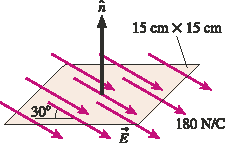
\includegraphics{figures/rk229.pdf}
\end{figure}

\item[\textbf{(24.11)}] Rafflæðið út um flötinn sem sést á myndinni er $\Phi_E = \SI{25}{Nm^2/C}$. Hver er styrkur rafsviðsins?

\begin{figure}[H]
    \centering
    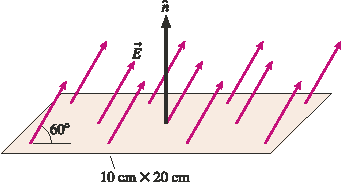
\includegraphics[scale = 0.8]{figures/rk2411.pdf}
\end{figure}

\item[\textbf{(24.16)}] Hvert er rafflæðið út um sívalningana hér fyrir neðan?

\begin{figure}[H]
    \centering
    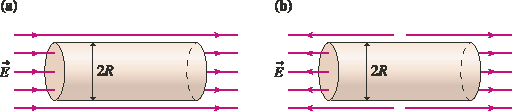
\includegraphics{figures/rk2416.pdf}
\end{figure}


\item[\textbf{(24.29)}] Ákarðið rafflæðin, $\Phi_1, \ldots, \Phi_5$ út um skábrettið hér fyrir neðan sem hallar um horn $\theta = \ang{30}$ og hefur hæð $h = \SI{2.0}{m}$ og breidd $b = \SI{4.0}{m}$. Styrkur rafsviðsins er $E = \SI{400}{N/C}$ í stefnu $x$-áss.

\begin{figure}[H]
    \centering
    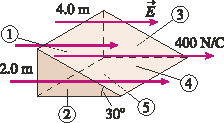
\includegraphics{figures/rk2429.pdf}
\end{figure}

\end{enumerate}

\begin{tcolorbox}
\begin{enumerate*}[label = \vspace{0.15cm} ]
  \item \textbf{(24.9)} $\Phi_E = \SI{-2.0}{Nm^2/C}$.
  \item \textbf{(24.11)} $\Phi_E = \SI{1400}{N/C}$.
  \item \textbf{(24.16)} $\Phi_a = 0$, $\Phi_b = 2E\pi r^2 $.
  \item \textbf{(24.29)} $\Phi_1 = \SI{-3200}{Nm^2/C}$, $\Phi_2 = \Phi_3 = \Phi_5 = \SI{0}{Nm^2/C}$, $\Phi_4 = \SI{3200}{Nm^2/C}$, $\Phi_{\text{heild}} = \SI{0}{Nm^2/C}$.
\end{enumerate*}
\end{tcolorbox}

\newpage

\subsection*{Dæmatími 5: Plötuþéttir}

\begin{tcolorbox}
Rafsviðið í plötuþétti er gefið með:
\begin{align*}
    E_{\text{plötuþéttir}} = \frac{Q}{\varepsilon_0 A}.
\end{align*}
Rafsviðslínurnar liggja frá jákvæðu plötunni og að neikvæðu plötunni.
\end{tcolorbox}

\begin{enumerate}[label = \textbf{(\alph*)}]

\item[\textbf{(23.3)}] Hver er styrkur og stefna rafsviðsins í svarta punktinum á myndinni?

\begin{figure}[H]
    \centering
    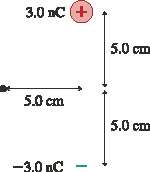
\includegraphics{figures/rk233.pdf}
\end{figure}

\item[\textbf{(23.23)}] Plötuþéttir samanstendur af tveimur diskum með þvermál $þ = \SI{6.0}{cm}$ í fjarlægð $d = \SI{2.0}{mm}$ frá hvor annarri. Styrkur rafsviðsins á milli platnanna er $\SI{1.0e6}{N/C}$. Hver er hleðslan á hvorri plötu?

\item[\textbf{(23.25)}] Tvær plötur eru í fjarlægð $d = \SI{1.0}{cm}$ frá hvor annarri og halda hleðslu $\pm q \gg e$. Nú er rafeind sleppt frá yfirborði neikvæðu plötunnar og róteind er sleppt á sama tíma frá yfirborði jákvæðu plötunnar. Hvar mætast rafeindin og róteindin?

\item[\textbf{(23.26)}] Tvær plötur með þvermál $þ = \SI{2.0}{cm}$ eru í fjarlægð $d = \SI{1.0}{mm}$ frá hvor annarri. Búið er að hlaða plöturnar í $q = \pm\SI{10}{nC}$. 
\begin{enumerate}[label = \textbf{(\alph*)}]
    \item Hvert er rafsviðið á milli platnanna?
    \item Róteind er skotið frá neikvæðu plötunni í átt að þeirri jákvæðu. Hver þarf upphafshraðinn að vera ef hún á rétt svo að sleikja yfirborð jákvæðu plötunnar?
\end{enumerate}

\end{enumerate}

\begin{tcolorbox}
\begin{enumerate*}[label = \vspace{0.15cm} ]
  \item \textbf{(23.3)} $\vec{E} = \smqty(0 \\ -7600) \, \si{N/C}$.
  \item \textbf{(23.23)} $Q = \SI{25}{nC}$.
  \item \textbf{(23.25)} $\ell_e = \SI{0.9995}{cm}$.
  \item \textbf{(23.26)} $E = \SI{3.6}{MN/C}$, $v = \SI{8.3e5}{m/s}$.
\end{enumerate*}
\end{tcolorbox}

\newpage

\subsection*{Dæmatími 6: Hreyfing í rafsviði}

\begin{tcolorbox}
Hreyfing í rafsviði er afar svipuð hreyfingu í þyngdarsviði. Kraftajafnan okkar verður þá:
\begin{align*}
    ma = qE, \hspace{0.9cm} \text{til samanburðar við:} \hspace{0.9cm} ma = mg
\end{align*}
Almennt þá gilda allar sömu stöðujöfnur og við höfðum lært fyrir einsleitt rafsvið, $E$. Núna er hröðunin bara $a = \frac{qE}{m}$ í staðinn fyrir $a = g$.
\end{tcolorbox}

\begin{enumerate}[label = \textbf{(\alph*)}]

\item[\textbf{(23.37)}] Hver er styrkur og stefna rafsviðsins í punktinum á myndinni?

\begin{figure}[H]
    \centering
    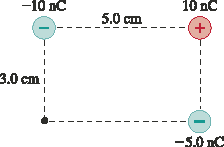
\includegraphics{figures/rk2337.pdf}
\end{figure}

\item[\textbf{(23.52)}] Rafeind er skotið undir horni $\theta = \ang{45}$ miðað ivð lárétt með upphafshraða $v_0 = \SI{5.0e6}{m/s}$ frá jákvæðu plötu plötuþéttisins eins og sést á myndinni hér fyrir neðan. Rafeindin lendir í fjarlægð $\ell = \SI{4.0}{cm}$ frá upphafsstaðsetningu sinni. \textbf{(a)} Hver er styrkur rafsviðsins inni í þéttinum? \textbf{(b)} Hvert er minnsata hugsanlega plötubilið, $d$?

\begin{figure}[H]
    \centering
    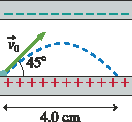
\includegraphics{figures/rk2352.pdf}
\end{figure}

\item[\textbf{(23.53)}] Rafeind er skotið frá jákvæðu plötu plötuþéttis undir horni $\theta = \ang{45}$ miðað við lárétt með upphafshraða $v_0$. Plötubilið er $d = \SI{2.0}{cm}$. Styrkur rafsviðsins er $E = \SI{1.0e4}{N/C}$. Hver er mesti hraðinn, $v_0$, sem að rafeindin getur haft án þess að rekast í neikvæðu plötuna?

\begin{figure}[H]
    \centering
    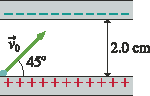
\includegraphics{figures/rk2353.pdf}
\end{figure}

\item[\textbf{(23.73)}] Skoðum hringlaga gjörð með geisla $R$ og jafndreifða hleðslu $Q$ sem liggur þannig að samhverfuás gjarðarinnar samsvarar $z$-ás hnitakerfisins. Nú er lítilli hleðslu $-q$ komið fyrir í $z = 0$ á samhverfuás gjarðarinnar. Nú er hleðslan færð um litla vegalengd $z$ frá jafnvægisstöðunni. Sýnið að fyrir $z \ll R$ þá verður tíðni einföldu sveifluhreyfingarinnar sem myndast við þetta gefin með:
\begin{align*}
    f = \frac{1}{2\pi} \sqrt{\frac{qQ}{4\pi \varepsilon_0 m R^3}}
\end{align*}

\end{enumerate}

\begin{tcolorbox}
\begin{enumerate*}[label = \vspace{0.15cm} ]
  \item \textbf{(23.37)} $\vec{E}_{\text{heild}} = \smqty(-4,7 \\ 86,4) \, \si{kN/C}$, $E_{\text{heild}} = \SI{86.5}{kN/C}$ og $\varphi = \SI{266.9}{\degree}$.
  \item \textbf{(23.52)} $d_{\text{max}} = \SI{9.9}{mm}$.
  \item \textbf{(23.53)} $v_0 = \SI{1.2e7}{m/s}$.
  \item \textbf{(23.73)} $m\Ddot{z} = - \frac{kQq}{R^3}z$, $\omega = \sqrt{\frac{kQq}{mR^3}}$, $f = \frac{\omega}{2\pi} = \SI{2.0e12}{Hz}$.
\end{enumerate*}
\end{tcolorbox}

\newpage

\subsection*{Dæmatími 7: Lögmál Gauss}


\begin{tcolorbox}
Lögmál Gauss segir að heildarrafflæðið út Gauss-flöt með rúmmál $V$ og yfirborðsflatarmál $A$ er:
\begin{align*}
    \Phi_{\text{heild}} = \oint \vec{E} \cdot d\vec{A} = \frac{Q_{\text{inni}}}{\varepsilon_0}
\end{align*}
Þar sem $Q_{\text{inni}}$ er heildarhleðslan sem að Gauss-flöturinn umlykur.
\end{tcolorbox}



\begin{enumerate}[label = \textbf{(\alph*)}]

\item[\textbf{(24.33)}] Hleðsla $q = +\SI{10}{nC}$ er stödd í miðjunni á jafnhliða tening með hliðarlengdir $\ell = \SI{2.0}{m}$. Hvert er rafflæðið út um efstu hlið kubbsins vegna hleðslunnar, $q$?

\item[\textbf{(24.43)}] Finnið rafsviðið \textbf{(a)} inni í \textbf{(b)} fyrir utan á sundbolta með geisla $R$ sem ber jafndreifða hleðslu $Q$ á yfirborðinu.

\item[\textbf{(24.54)}] Lítum á kúluskel með innri geisla $a$ og ytri geisla $b$. Hleðslan, $Q$, í kúluskelinni er jafndreifð um rúmmál hennar. Kúluskelin er hol að innan fyrir $r < a$.
\begin{enumerate}[label = \textbf{(\alph*)}]
    \item Hvert er rafsviðið fyrir $r \geq b$?
    \item Hvert er rafsviðið fyrir $r < a$?
    \item Hvert er rafsviðið fyrir $a < r < b$?
\end{enumerate}

\item[\textbf{(24.55)}] Eitt af fyrstu atómlíkönum Rutherfords hafði kjarna með hleðslu $+Ze$ í miðjunni (fjöldi róteindanna var þá heiltalan $Z$) og jafndreifða neikvæða hleðslu $-Ze$ í rúmmáli kúlu með geisla $R$.
\begin{enumerate}[label = \textbf{(\alph*)}]
    \item Sýnið að rafsviðið inni í atóminu ($r < R$) er:
    \begin{align*}
        E = \frac{Ze}{4\pi \varepsilon_0} \left( \frac{1}{r^2} - \frac{r}{R^3} \right).
    \end{align*}
    \item Hvert er gildið á $E$ við yfirborð atómsins?
    \item Úran hefur $Z = 92$ róteindir og geisla $R = \SI{0.10}{nm}$. Hver er rafsviðsstyrkurinn inni í Úranatómi í $r = \frac{1}{2}R$ fjarlægð frá kjarnanum?
\end{enumerate}


\end{enumerate}

\begin{tcolorbox}
\begin{enumerate*}[label = \vspace{0.15cm} ]
  \item \textbf{(24.33)} $\Phi_{\text{toppur}} = \SI{190}{Nm^2/C}$.
  \item \textbf{(24.43)} $\displaystyle E(r) = \begin{cases} 0 & \text{ef $r<R$} \\[0.5pt] \frac{Q}{4\pi \varepsilon_0 r^2} & \text{ef $r \geq R$} \end{cases}$
  \item \textbf{(24.54)} $\displaystyle E(r) = \begin{cases} 0 & \text{ef $r < a$} \\[0.75pt] \frac{Q}{4\pi \varepsilon_0 r^2} \cdot \frac{r^3-a^3}{b^3-a^3} & \text{ef $a \leq r \leq b$} \\[0.75pt] \frac{Q}{4\pi \varepsilon_0 r^2} & \text{ef $r < b$} \end{cases}$
  \item \textbf{(24.55)} $E(r) = \frac{Ze}{4\pi \varepsilon_0} \cdot \left( \frac{1}{r^2} - \frac{r}{R^3} \right)$, $E(R) = 0$, $E_U(\frac{1}{2}R) = \SI{4.6e23}{N/C}$.
\end{enumerate*}
\end{tcolorbox}


\newpage




%%%%%%%%%%%%%%%%%%%%%%%%%%%%%%%%
%      END OF CHAPTER TEXT 
%%%%%%%%%%%%%%%%%%%%%%%%%%%%%%%%
\ifdefined \wholebook \else
 \printindex
\end{document}
\fi
